% -*- latex -*-
%%%%%%%%%%%%%%%%%%%%%%%%%%%%%%%%%%%%%%%%%%%%%%%%%%%%%%%%%%%%%%%%
%%%%%%%%%%%%%%%%%%%%%%%%%%%%%%%%%%%%%%%%%%%%%%%%%%%%%%%%%%%%%%%%
%%%%
%%%% This text file is part of the source of 
%%%% `Parallel Programming in MPI and OpenMP'
%%%% by Victor Eijkhout, copyright 2012-2020
%%%%
%%%% mpi-topo.tex : about communicator topologies
%%%%
%%%%%%%%%%%%%%%%%%%%%%%%%%%%%%%%%%%%%%%%%%%%%%%%%%%%%%%%%%%%%%%%
%%%%%%%%%%%%%%%%%%%%%%%%%%%%%%%%%%%%%%%%%%%%%%%%%%%%%%%%%%%%%%%%

A communicator describes a group of processes, but the structure of
your computation may not be such that every process will communicate
with every other process. For instance, in a computation that is
mathematically defined on a
Cartesian 2D grid, the
processes themselves act as if they are two-dimensionally ordered and communicate
with N/S/E/W neighbours. If MPI had this knowledge about your
application, it could conceivably optimize for it, for instance by
renumbering the ranks so that communicating processes are closer
together physically in your cluster.

The mechanism to declare this structure of a computation to MPI
is known as a \indextermsub{virtual}{topology}. The following types of
topology are defined:
\begin{itemize}
\item \indexmpishow{MPI_UNDEFINED}: this values holds for communicators where no
  topology has explicitly been specified.
\item \indexmpishow{MPI_CART}: this value holds for Cartesian
  toppologies, where processes act as if they are ordered in a
  multi-dimensional `brick'; see
  section~\ref{sec:cartesian}.
\item \indexmpishow{MPI_GRAPH}: this value describes the graph
  topology that was defined in \indextermbus{MPI}{1};
  section~\ref{sec:mpi-1-graph}. It is unnecessarily burdensome, since
  each process needs to know the total graph, and should therefore be
  considered obsolete; the type \indexmpishow{MPI_DIST_GRAPH} should
  be used instead.
\item \indexmpishow{MPI_DIST_GRAPH}: this value describes the distributed graph
  topology where each process only describes the edges in the process
  graph that touch itself; see section~\ref{sec:mpi-dist-graph}.
\end{itemize}
These values can be discovered with the routine
\indexmpiref{MPI_Topo_test}.

\Level 0 {Cartesian grid topology}
\label{sec:cartesian}

A \indextermsub{Cartesian}{grid} is a structure, typically in 2~or~3 dimensions,
of points that have two neighbours in each of the dimensions.
Thus, if a Cartesian grid has sizes $K\times M\times N$, its
points have coordinates $(k,m,n)$ with $0\leq k<K$ et cetera.
Most points have six neighbours $(k\pm1,m,n)$, $(k,m\pm1,n)$, $(k,m,n\pm1)$;
the exception are the edge points. A~grid where edge processors
are connected through \indexterm{wraparound connections} is called
a \indextermsub{periodic}{grid}.

The most common use of Cartesian coordinates
is to find the rank of process by referring to it in grid terms.
For instance, one could ask `what are my neighbours offset by $(1,0,0)$, 
$(-1,0,0)$, $(0,1,0)$ et cetera'.

While the Cartesian topology interface is fairly easy to use, as
opposed to the more complicated general graph topology below, it is
not actually sufficient for all Cartesian graph uses. Notably, in
a so-called \indextermsub{star}{stencil}, such as the
\indextermsub{nine-point}{stencil}, there are diagonal connections,
which can not be described in a single step. Instead, it is necessary
to take a separate step along each coordinate dimension. In higher
dimensions this is of course fairly awkward.

Thus, even for Cartesian structures, it may be advisable to use the
general graph topology interface.

\Level 1 {Cartesian routines}

The cartesian topology is specified by giving
\indexmpishow{MPI_Cart_create} the sizes of the processor grid along
each axis, and whether the grid is periodic along that axis.

\lstset{style=reviewcode,language=C} %pyskip
\begin{lstlisting}
int MPI_Cart_create(
  MPI_Comm comm_old, int ndims, int *dims, int *periods, 
  int reorder, MPI_Comm *comm_cart)
\end{lstlisting}

Each point in this new communicator has a coordinate and a rank.  They
can be queried with \indexmpishow{MPI_Cart_coords} and
\indexmpishow{MPI_Cart_rank} respectively.

\lstset{style=reviewcode,language=C} %pyskip
\begin{lstlisting}
int MPI_Cart_coords(
  MPI_Comm comm, int rank, int maxdims,
  int *coords);
int MPI_Cart_rank(
  MPI_Comm comm, init *coords, 
  int *rank);
\end{lstlisting}

Note that these routines can give the coordinates for any rank,
not just for the current process.
%
\cverbatimsnippet{cart}

The \n{reorder} parameter to \indexmpishow{MPI_Cart_create}
indicates whether processes can have a rank
in the new communicator that is different from in the old one.

Strangely enough you can only shift in one direction, you can not
specify a shift vector.
\begin{lstlisting}
int MPI_Cart_shift(MPI_Comm comm, int direction, int displ, int *source, 
                  int *dest)
\end{lstlisting}
If you specify a processor outside the grid
the result is \indexmpishow{MPI_PROC_NULL}.

\cverbatimsnippet{cartshift}

\Level 0 {Distributed graph topology}
\label{sec:mpi-dist-graph}

\begin{figure}
  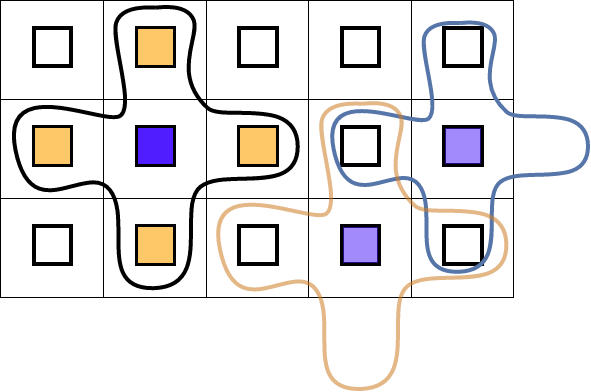
\includegraphics[scale=.5]{graphcollective}
  \caption{Illustration of a distributed graph topology where each
    node has four neighbours}
  \label{fig:graphcollective}
\end{figure}

In many calculations on a grid (using the term in its mathematical,
\ac{FEM}, sense), a grid point will collect information from grid
points around it. Under a sensible distribution of the grid over
processes, this means that each process will collect information from
a number of neighbour processes. The number of 
neighbours is dependent on that process. For instance, in a 2D
grid (and assuming a five-point stencil for the computation) most
processes communicate with four neighbours; processes on the edge with
three, and processes in the corners with two.

Such a topology is illustrated in figure~\ref{fig:graphcollective}.

MPI's notion of \indextermbusdef{graph}{topology}, and the
\indextermsubdef{neighbourhood}{collectives}, offer an elegant way of
expressing such communication structures. There are various reasons
for using graph topologies over the older, simpler methods.
\begin{itemize}
\item MPI is allowed to reorder the ranks, so that network proximity
  in the cluster corresponds to proximity in the structure of the
  code.
\item Ordinary collectives could not directly be used for graph
  problems, unless one would adopt a subcommunicator for each graph
  neighbourhood. However, scheduling would then lead to deadlock or
  serialization.
\item The normal way of dealing with graph problems is through
  non-blocking communications. However, since the user indicates an
  explicit order in which they are posted, congestion at certain
  processes may occur.
\item Collectives can pipeline data, while send/receive operations
  need to transfer their data in its entirety.
\item Collectives can use spanning trees, while send/receive uses a
  direct connection.
\end{itemize}

Thus the minimal description of a process graph contains for each process:
\begin{itemize}
\item Degree: the number of neighbour processes; and
\item the ranks of the processes to communicate with.
\end{itemize}
However, this ignores that communication is not always symmetric:
maybe the processes you receive from are not the ones you send
to. Worse, maybe only one side of this duality is easily
described. Therefore, there are two routines:
\begin{itemize}
\item \indexmpishow{MPI_Dist_graph_create_adjacent} assumes that a
  process knows both who it is sending it, and who will send to
  it. This is the most work for the programmer to specify, but it is
  ultimately the most efficient.
\item \indexmpishow{MPI_Dist_graph_create} specifies on each process
  only what it is the source for; that is, who this process will be sending
  to. Consequently, some amount of processing
  --~including communication~-- is needed to build the converse
  information, the ranks that will be sending to a process.
\end{itemize}

\Level 1 {Graph creation}

There are two creation routines for process graphs. These routines are
fairly general in that they allow any process to specify any part of
the topology. In practice, of course, you will mostly let each process
describe its own neighbour structure.

The routine \indexmpishow{MPI_Dist_graph_create_adjacent} assumes that a process
knows both who it is sending it, and who will send to it. This means
that every edge in the communication graph is represented twice, so
the memory footprint is double of what is strictly necessary. However,
no communication is needed to build the graph.

The second creation routine, \indexmpiref{MPI_Dist_graph_create}, is
probably easier to use, especially in cases where the communication
structure of your program is symmetric, meaning that a process sends
to the same neighbours that it receives from.  Now you specify on each
process only what it is the source for; that is, who this process will
be sending to.\footnote{I disagree with this design
  decision. Specifying your sources is usually easier than specifying
  your destinations.}. Consequently, some amount of processing
--~including communication~-- is needed to build the converse
information, the ranks that will be sending to a process.

Figure~\ref{fig:graphcollective} describes the common five-point
stencil structure. If we let each process only describe itself, we get
the following:
\begin{itemize}
\item \n{nsources}$=1$ because the calling process describes on node
  in the graph: itself.
\item \n{sources} is an array of length~1, containing the rank of the
  calling process.
\item \n{degrees} is an array of length~1, containing the degree
  (probably:~4) of this process.
\item \n{destinations} is an array of length the degree of this
  process, probably again~4. The elements of this array are the ranks
  of the neighbour nodes; strictly speaking the ones that this process
  will send to.
\item \n{weights} is an array declaring the relative importance of the
  destinations. For an \indextermsub{unweighted}{graph} use
  \indexmpishow{MPI_UNWEIGHTED}.
\item \n{reorder} (\n{int} in~C, \n{LOGICAL} in~Fortran) indicates
  whether MPI is allowed to shuffle ranks to achieve greater locality.
\end{itemize}

The resulting communicator has all the processes of the original
communicator, with the same ranks. Its main point is usage in the
so-called `neighbour collectives'.

\Level 1 {Neighbour collectives}

We can now use the graph topology to perform a gather or allgather
\indexmpiref{MPI_Neighbor_allgather}
that combines only the processes directly connected to the calling
process.

The neighbour collectives have the same argument list as the regular
collectives, but they apply to a graph communicator.

\begin{figure}[ht]
  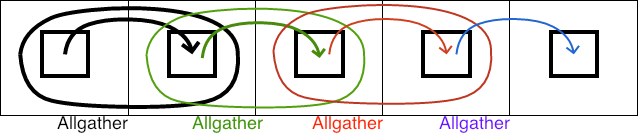
\includegraphics[scale=.5]{rightgraph}
  \caption{Solving the right-send exercise with neighbourhood
    collectives}
  \label{fig:rightgraph}
\end{figure}

\begin{exercise}
  \label{ex:rightgraph}
  Revisit exercise~\ref{ex:serialsend} and solve it using
  \indexmpishow{MPI_Dist_graph_create}. Use figure~\ref{fig:rightgraph} for inspiration.
\end{exercise}

The other collective is \indexmpishow{MPI_Neighbor_alltoall}.

The vector variants are
\indexmpishow{MPI_Neighbor_allgatherv}
and
\indexmpishow{MPI_Neighbor_alltoallv}.

There is a heterogenous (multiple datatypes) variant:
\indexmpishow{MPI_Neighbor_alltoallw}.

For unclear reasons there is no \indexmpishow{MPI_Neighbor_allreduce}.

\Level 1 {Query}

Statistics query:
%
\indexmpishow{MPI_Dist_graph_neighbors_count}
%
\indexmpishow{MPI_Dist_graph_neighbors_count}

\Level 1 {Graph topology (deprecated)}
\label{sec:mpi-1-graph}

The original \indextermbus{MPI}{1} had a graph topology interface
\indexmpidef{MPI_Graph_create}
which required each process to specify the full process graph. Since
this is not scalable, it should be considered deprecated. Use the
distributed graph topology (section~\ref{sec:mpi-dist-graph}) instead.

Other legacy routines: 
\indexmpidef{MPI_Graph_neighbors},
\indexmpidef{MPI_Graph_neighbors_count},
\indexmpidef{MPI_Graph_get},
\indexmpidef{MPI_Graphdims_get}.
